\section {Results}
\label{results}

\subsection {Analysis}
First, we will start by showing that without machine learning, we'd have to select a gene that works best for the task at hand. Then, we will demonstrate how that selection compares to random mean absolute error (MAE) and to baseline MAE. We will then move on to improving this performance by using machine learning with a perceptron model, an MLP, and bagging.

\subsubsection{Interpretation Guide}
Note that MAE corresponds directly to the average distance from gold standard in units of words. For exmample, an $MAE < 50$ means that on average, the algorithm is within 50 words of the correct position. Baseline varies according to type, but on average, it is approx. 150.

\subsection{Selecting the Best Genetic Algorithm: Error By Imitation Class}
Figure \ref{fig:totalErrorAll} shows how each gene performs across all imitation types. No matter what which gene was used, the lowest MAE was achieved for type 1 imitations. This seems to indicate that type 1 imitations are easiest to locate. Figure \ref{fig:c1} shows the same information as Figure \ref{fig:totalErrorAll}, but focuses on showing MAE for type 1 imitations, adding in baseline and random MAE, both of which are beat by every gene.

Figure \ref{fig:overall} shows the average MAE for each gene. Overall, gene 1 is best, but only by a small margin. Genes 3, 5, and 7 could probably be selected as well. However, due to the simplicity of gene 1 and the fact that it achieved the lowest MAE in every trial, it would be selected if we had to choose one gene only \footnote{We do not have to settle for any 1 gene since machine learning handle the meta-data from multiple genes at a time}. Table \ref{tab:best-for-each} reports the MAE for each citation type explicitly. Since our task aims to minimize MAE for all imitation types, we will focus on beating the average MAE of $99.41$. The worst gene was number 8, having an MAE of $107.82$. 

\begin{figure}[center]
	\centering
	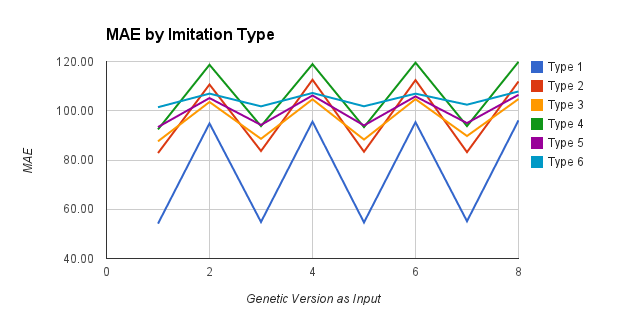
\includegraphics[width=16cm]{images/total_error_all_approaches.png}
	\caption{Type 1 imitations are always lowest, no matter the gene. The up-down pattern is caused by reversing of genes, which was turned on for even runs of genetic alignment. }
	\label{fig:totalErrorAll}
\end{figure}

\begin{figure}[center]
	\centering
	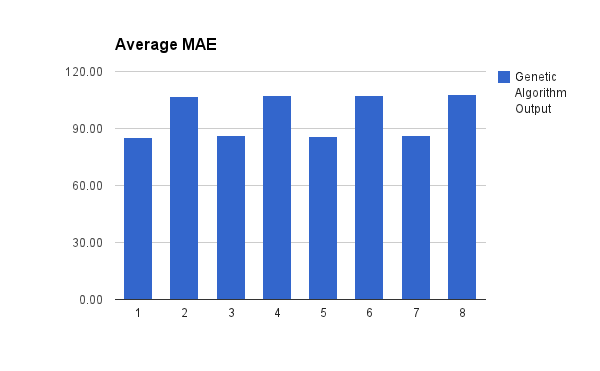
\includegraphics[width=16cm]{images/average_MAE.png}
	\caption{Gene 1 is best, but genes 3, 5, and 7 are comparable. The other four cases all have the reversing turned on. Reversing was not beneficial to MAE.}
	\label{fig:overall}
\end{figure}

\begin{figure}[center]
	\centering
	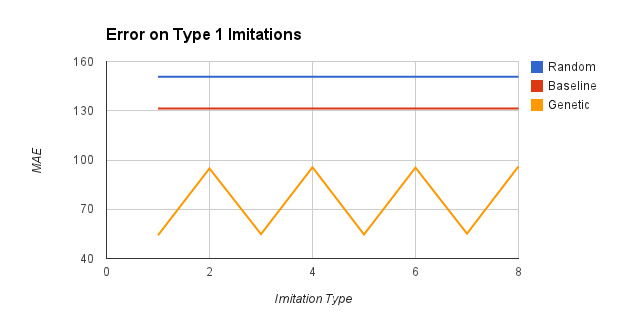
\includegraphics[width=16cm]{images/error_type_1_imitations.png}
	\caption{No matter which gene is used, improvement over baseline is achieved.}
	\label{fig:c1}
\end{figure}

\begin{table}[center]
	\centering
	\begin{center}
		\begin{tabular}{|l|c|} \hline
			\textbf{Imitation Type}	&	{MAE}		\\ \hline \hline
			1			&	54.15		\\ \hline
			2			&	82.81		\\ \hline
			3			&	87.59		\\ \hline
			4			&	92.42		\\ \hline
			5			&	93.38		\\ \hline
			6			&	101.43		\\ \hline
			Average of 1-6		&	99.41		\\ \hline
		\end{tabular}
	\end{center}
	\caption{MAE for genetic algorithm 1.}
	\label{tab:best-for-each}
\end{table}

\clearpage

\subsection{ML Models Compared}
Recall that we have 8 genes to work with. We use each as input to various machine learning (ML) models and chart the resulting MAE in Figure \ref{fig:mae_by_type}. Since our machine learning models can handle many inputs, we also provided all meta-data we could obtain from all genes for another set of training runs for each ML model. We labeled this as 0 on the `Genetic Version as Input' axis. 

The perceptron, in some cases, performed worse than the genes themselves, but when provided all genes as input, it did outperform the genes themselves. In fact, every ML model achieved it's lowest MAE when provided the meta-data of multiple genes. Bagging was best with an MAE of $80.15$, which is about 20\% closer to gold than the gene itself! MLP performed more poorly, but almost always outperforms the perceptron. It probably would have outperformed the perceptron more often if we had found a better settings for it, but it was so slow to learn that it just wasn't worth it. Bagging, on the other hand, was significantly faster and yielded great results.

\begin{figure}[center]
	\centering
	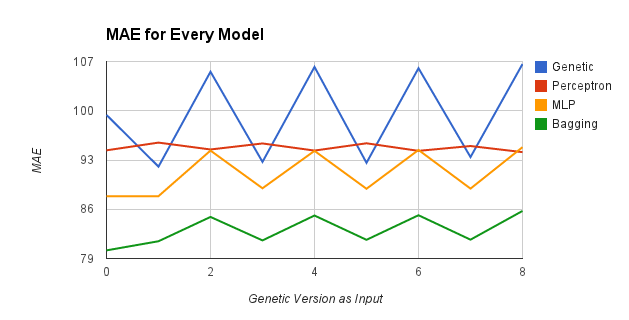
\includegraphics[width=16cm]{images/MAE_by_type.png}
	\caption{Overall MAE of all models compared. Gene 0 is a combination of genes 1-8 for the ML models. For the genetic model, gene 0 is the average MAE for genes 1-8.}
	\label{fig:mae_by_type}
\end{figure}
